% Template for Elsevier CRC journal article
% version 1.2 dated 09 May 2011

% This file (c) 2009-2011 Elsevier Ltd.  Modifications may be freely made,
% provided the edited file is saved under a different name

% This file contains modifications for Transportation Research Procedia

% Changes since version 1.1
% - added "procedia" option compliant with ecrc.sty version 1.2a
%   (makes the layout approximately the same as the Word CRC template)
% - added example for generating copyright line in abstract

%-----------------------------------------------------------------------------------

%% This template uses the elsarticle.cls document class and the extension package ecrc.sty
%% For full documentation on usage of elsarticle.cls, consult the documentation "elsdoc.pdf"
%% Further resources available at http://www.elsevier.com/latex

%-----------------------------------------------------------------------------------

%%%%%%%%%%%%%%%%%%%%%%%%%%%%%%%%%%%%%%%%%%%%%%%%%%%%%%%%%%%%%%
%%%%%%%%%%%%%%%%%%%%%%%%%%%%%%%%%%%%%%%%%%%%%%%%%%%%%%%%%%%%%%
%%                                                          %%
%% Important note on usage                                  %%
%% -----------------------                                  %%
%% This file should normally be compiled with PDFLaTeX      %%
%% Using standard LaTeX should work but may produce clashes %%
%%                                                          %%
%%%%%%%%%%%%%%%%%%%%%%%%%%%%%%%%%%%%%%%%%%%%%%%%%%%%%%%%%%%%%%
%%%%%%%%%%%%%%%%%%%%%%%%%%%%%%%%%%%%%%%%%%%%%%%%%%%%%%%%%%%%%%

%% The '3p' and 'times' class options of elsarticle are used for Elsevier CRC
%% The 'procedia' option causes ecrc to approximate to the Word template
\documentclass[5p,times,procedia]{elsarticle}
\flushbottom

%% The `ecrc' package must be called to make the CRC functionality available
\usepackage{ecrc}
\usepackage{amsmath}
\usepackage[utf8]{inputenc}
\usepackage[mode=buildnew]{standalone}% requires -shell-escape
\usepackage{tikz}
\usepackage{pgfplots}
\usepackage{booktabs}
\usepackage{adjustbox}
\usepackage{multirow}
\usepackage{caption}
\usepackage{subcaption}
\usepgfplotslibrary{groupplots}
\usepgfplotslibrary{dateplot}
\pgfplotsset{compat=newest}

%% The ecrc package defines commands needed for running heads and logos.
%% For running heads, you can set the journal name, the volume, the starting page and the authors

%% set the volume if you know. Otherwise `00'
\volume{00}

%% set the starting page if not 1
\firstpage{1}

%% Give the name of the journal
\journalname{Procedia CIRP}

%% Give the author list to appear in the running head
%% Example \runauth{C.V. Radhakrishnan et al.}
\runauth{Author name}

%% The choice of journal logo is determined by the \jid and \jnltitlelogo commands.
%% A user-supplied logo with the name <\jid>logo.pdf will be inserted if present.
%% e.g. if \jid{yspmi} the system will look for a file yspmilogo.pdf
%% Otherwise the content of \jnltitlelogo will be set between horizontal lines as a default logo

%% Give the abbreviation of the Journal.
\jid{trpro}

%% Give a short journal name for the dummy logo (if needed)
%\jnltitlelogo{Transportation Research}

%% Hereafter the template follows `elsarticle'.
%% For more details see the existing template files elsarticle-template-harv.tex and elsarticle-template-num.tex.

%% Elsevier CRC generally uses a numbered reference style
%% For this, the conventions of elsarticle-template-num.tex should be followed (included below)
%% If using BibTeX, use the style file elsarticle-num.bst

%% End of ecrc-specific commands
%%%%%%%%%%%%%%%%%%%%%%%%%%%%%%%%%%%%%%%%%%%%%%%%%%%%%%%%%%%%%%%%%%%%%%%%%%

%% The amssymb package provides various useful mathematical symbols

\usepackage{amssymb}
%% The amsthm package provides extended theorem environments
%% \usepackage{amsthm}

%% The lineno packages adds line numbers. Start line numbering with
%% \begin{linenumbers}, end it with \end{linenumbers}. Or switch it on
%% for the whole article with \linenumbers after \end{frontmatter}.
%% \usepackage{lineno}

%% natbib.sty is loaded by default. However, natbib options can be
%% provided with \biboptions{...} command. Following options are
%% valid:

%%   round  -  round parentheses are used (default)
%%   square -  square brackets are used   [option]
%%   curly  -  curly braces are used      {option}
%%   angle  -  angle brackets are used    <option>
%%   semicolon  -  multiple citations separated by semi-colon
%%   colon  - same as semicolon, an earlier confusion
%%   comma  -  separated by comma
%%   numbers-  selects numerical citations
%%   super  -  numerical citations as superscripts
%%   sort   -  sorts multiple citations according to order in ref. list
%%   sort&compress   -  like sort, but also compresses numerical citations
%%   compress - compresses without sorting
%%
%\biboptions{authoryear}

% \biboptions{}

% if you have landscape tables
\usepackage[figuresright]{rotating}
%\usepackage{harvard}
% put your own definitions here:x
%   \newcommand{\cZ}{\cal{Z}}
%   \newtheorem{def}{Definition}[section]
%   ...

% add words to TeX's hyphenation exception list
%\hyphenation{author another created financial paper re-commend-ed Post-Script}

% declarations for front matter

\usepackage[bookmarks=false]{hyperref}
    \hypersetup{colorlinks,
      linkcolor=blue,
      citecolor=blue,
      urlcolor=blue}
\usepackage{xcolor}
\newcommand{\AP}[1]{{\color{blue} {\bf (AP: #1)}}}
\newcommand{\LS}[1]{{\color{purple} {\bf (LS: #1)}}}
\newcommand{\FS}[1]{{\color{cyan} {\bf (FS: #1)}}}
\newcommand{\MW}[1]{{\color{teal} {\bf (MW: #1)}}}
\newcommand{\JG}[1]{{\color{green} {\bf (JG: #1)}}}
\newcommand{\DSt}[1]{{\color{orange} {\bf (DSt: #1)}}}

\begin{document}
\begin{frontmatter}

%% Title, authors and addresses

%% use the tnoteref command within \title for footnotes;
%% use the tnotetext command for the associated footnote;
%% use the fnref command within \author or \address for footnotes;
%% use the fntext command for the associated footnote;
%% use the corref command within \author for corresponding author footnotes;
%% use the cortext command for the associated footnote;
%% use the ead command for the email address,
%% and the form \ead[url] for the home page:
%%
%% \title{Title\tnoteref{label1}}
%% \tnotetext[label1]{}
%% \author{Name\corref{cor1}\fnref{label2}}
%% \ead{email address}
%% \ead[url]{home page}
%% \fntext[label2]{}
%% \cortext[cor1]{}
%% \address{Address\fnref{label3}}
%% \fntext[label3]{}

\dochead{54th CIRP Conference on Manufacturing Systems}%

\title{Predictive analytics in quality assurance for assembly processes:
       lessons learned from a case study at an industry 4.0 demonstration cell}

%% use optional labels to link authors explicitly to addresses:
%% \author[label1,label2]{<author name>}
%% \address[label1]{<address>}
%% \address[label2]{<address>}



\author[a]{Peter Burggräf}
\author[a]{Johannes Wagner}
\author[a]{Benjamin Koke}
\author[a]{Fabian Steinberg} 
\author[a]{Alejandro R. Pérez M.*}
\author[a]{Lennart Schmallenbach}
\author[b,c]{Jochen Garcke}
\author[b]{Daniela Steffes-lai}
\author[b,d]{Moritz Wolter}

%\ead{author@institute.xxx}

\address[a]{Chair of International Production Engineering and Management (IPEM), Universität Siegen, Paul-Bonatz-Straße 9-11, Siegen - 57076, Germany}
\address[b]{Fraunhofer Institute for Algorithms and Scientific Computing (SCAI), Schloss Birlinghoven 1, Sankt Augustin- 53757, Germany}
\address[c]{Institut for Numerical Simulation, Universität Bonn, Endenicher Allee 19b, 53115 Bonn}
\address[d]{Institut for Computer Science, Universität Bonn, Endenicher Allee 19a, 53115 Bonn}

\aucores{* Corresponding author. Tel.: +49-271-740-4509; fax: +49-271-740-2630. {\it E-mail address:} alejandro.perez@uni-siegen.de}

\begin{abstract}
%% Text of abstract
Quality assurance (QA) is an important task in manufacturing to assess whether products 
meet their specifications. However, QA might be expensive, time-consuming, incomplete, or delayed.
This paper presents a solution for predictive analytics in QA based on machine sensor values during
production while employing machine-learning models based on logistic regression in a controlled environment. 
Furthermore, we present lessons learned while implementing this model, which helps to reduce complexity in
further industrial applications. The paper’s outcome proves that the developed model was able to predict
product quality, as well as to identify the correlation between machine-status and faulty product occurrence.
\end{abstract}

\begin{keyword}
Machine-Learning \sep Predictive Quality \sep Production \sep Quality Assurance \sep Logistic Regression 

%% keywords here, in the form: keyword \sep keyword

%% PACS codes here, in the form: \PACS code \sep code

%% MSC codes here, in the form: \MSC code \sep code
%% or \MSC[2008] code \sep code (2000 is the default)

\end{keyword}
%\cortext[cor1]{Corresponding author. Tel.: +0-000-000-0000 ; fax: +0-000-000-0000.}

\end{frontmatter}


\section{Introduction} % 1 Page (incl authors, abstract)

Product features such as reliability, durability, or complete functionality determine to a large extent the success and profit of companies on the market. That is why it is highly important for companies to ensure that every product meet the expected requirements. Throughout the years, diverse methods for quality control (QC) have been presented and implemented in production. Some of those methods prove to be highly effective, but costly, i.e. the revision of every produced piece, either by automated or manual methods, or by doing quality inspections based on a portion of the produced pieces and extend the results based on statistical methods. Which still has a considerable risk of not detecting NOK parts and sending them to costumers \cite{mitra2016fundamentals, fox1993quality, kahle2013zuverlaessigkeitsanalyse}.

Whenever a QC method is selected, it is important to remark that compromises must be made in most cases. For example, traditional methods like controlling every produced piece might affect the production goals by delaying the production speed at the cost of lower rejection rates On the other hand, higher production speeds normally requires statistical quality control methods. However, those methods do not provide one hundred percent certainty that the required product quality will be achieved \cite{selvamuthu2018introduction, kurniati2015quality}.

With the evolution of machine learning (ML) applications, we expect to enhance the QC by predicting the product quality at the initial stage of production. This will not only reduce cost in production, and strengthen the QC process, it will also be part of the predictive analytics tools found in production, which is currently widely used in diverse fields due to its accurate predictions \cite{bishop2006pattern, krauss2019machine}.

This paper is divided in 6 sections:

\begin{itemize}
       \item \textbf{Introduction}, states the motivation of the project as well as the problem it intended to be addressed.
       \item \textbf{Related Works}, covers the methods used in quality check in production, as well as the bases of predictive analytics in production.
       \item \textbf{The case industry 4.0 demonstration cell}, describe the demonstration cell used on this project. It answer the question of where to test predictive analytics in a controlled environment and why our system is a valid platform for this implementation.
       \item \textbf{Machine learning Methods}, explains the three machine learning methods implemented on this work: Multilayer perceptrons, Support Vector Machines, Decision Tree.
       \item \textbf{Experiments}, describe the experiment process from the data acquisition and preprocessing, to the classifier optimization and testing.
       \item \textbf{Conclusion}, express the remarks and diskoveries achieved after the finalization of this project phase, as well as presents a list of lessons learned during the implementation of the project, which might be helpful on further implementations.
\end{itemize}

\section{Related Works} % 1 Page \Lennart

\subsection{Quality check in production} \label{sec:qcp} % Basic books (find summarize) basic concepts 


The quality control of production processes and products is one fundamental part of general quality management. It contains the measures and activities needed to fulfill specific quality requirements \cite{illes2017new}.
According to Illés, there are three established tools and methods of quality control \cite{illes2017new}:
The Statistical Process Control (SPC), Auditing and Total Quality Control (TQC).   
The SPC is normally used to monitor the production process using recorded data values for the quality characteristics, as well as to indicate any significant changes in the quality characteristics in the production process \cite{selvamuthu2018introduction}. SPC methods can also take place before the actual manufacturing process, this is commonly known as "off-line SPC". 

During the design phase of a process or product, off-line SPC procedures are deployed. Those procedures aim to increase the quality of the outcoming product by choosing controllable products and  process parameter \cite{mitra2016fundamentals}.

The biggest advantage of working with SPC is that large batches can be checked without major time impact on the QC process, however, this would be only possible if the variance of the process product parameters is small enough, to ensure process capability \cite{kahle2013zuverlaessigkeitsanalyse}.

Another conservative technique to perform the quality check would be to check 100\% of the produced parts. On this method, every product is controlled and binary sorted as an OK or Non-OK part. However, this has the disadvantage of high cost related to personal or specialized material and in certain cases, could lead to a delay in production.

Product and process auditing is the independent examination of product and process quality to provide information and it is considered the most fundamental quality control technique. This method is executed by
an independent auditor, who based on sampling or checking records limits the finding on reporting incorrect processes procedures or products documentation. In a further step, the findings would be later corrected by another person rather than the auditor \cite{fox1993quality}. 

%Both statistical methods and hundred percent controls can be applied as an audit tool.

Statistical methods such as acceptance sampling or quality control charts represent a compromise between zero and the hundred percent control \cite{selvamuthu2018introduction, kurniati2015quality}.

While the SPC mostly optimizes the capability of the process, for example the acceptance plan prevents the nonconforming product to be pass and then delivered to the next process or the customer \cite{kurniati2015quality}.
In the case of a hundred percent control, this is associated with higher costs and a higher requirement of time, compared to a quality control based on a machine learning model.
Generally, statistical methods are faster than the hundred percent controls, however, their disadvantage is that those methods are based on assumptions. those assumptions might lead to errors if the variance of the product quality higher than expected.

The concept of TQC is to extend the scope of quality control to the whole company and product life cycle, by involving all departments of the organization \cite{illes2017new}.
The quality characteristics of a product can be classified as variables or attributes.
Variables are measurable characteristics, which are shown as numbers. On the contrary, attributes are not measurable and can only take the binary values like "go" or "no-go" \cite{mitra2016fundamentals}. 
The advantage of variable measurements is that in the event of a defective intermediate or end product, precise measured values are available, which enable precise adjustment of the process parameters. 
This allows the desired quality to be restored. With that in mind, predictive quality control is a promising solution.

\subsection{Predictive analytics in production}

According to Delen and Damirkan, predictive analytics (PA) consist on unravel the inherent relationships (if any) between input and output by using data and mathematical techniques \cite{delen2013data}.

PA offers a wide range of applications, and it can be implemented as long as there is enough data available. By considering the industrial and production environment, PA would be a great asset due to the high flexibility and high amount of data available coming from processes, single machines or cells, products, and others. Some common industrial applications of PA at the industry are focused products (design and optimization), machines (predictive maintenance) and production (scheduling) \cite{krauss2019machine}.

Applications that combines PA with QC might be a great improvement in the quality control process because it is an improvement compared with the earlier mentioned methods \ref{sec:qcp}, in terms of speed, accuracy and time delay. 

The outcome of an explorative literature review on this matter, shows that the findings that combines PA and QC are very scarce in the literature. This could be in great part, due to the novelty of the area \cite{aumi2012model, ritter1992neue}. Related work, e.g from Krauß focused on automated machine learning for predictive quality in production \cite{krauss2020automated} and a product quality prediction in a process chain \cite{krauss2019machine}. 

Based on an explorative literature review on this matter, the short outcome is that the findings that combine PA and QC are very scarce in the literature. This could be in great part, due to computer power limitations in early research and the recent increase of ML applications on this area. Related works, e.g from Krauß focused on automated machine learning for predictive quality in production \cite{krauss2020automated}; product quality prediction in a process chain \cite{krauss2019machine}; model development for predictive quality control of batch processes \cite{aumi2012model}; and ways of process modeling on quality prediction and assurance of chipboard \cite{ritter1992neue}. Considering the lack of literature, our goal is to decrease this gap on the research area by implementing a functional predictive model in quality assurance for an assembly process, as well as describing the lesson learned during this implementation.
       
\section{The case industry 4.0 demonstration cell} % (taken from title) % 3/4 Page

To test our theories, we need to select the right testing platform. This platform should represent real industrial applications and be able to handle a certain level of complexity. In our work, we applied a case-based research approach \cite{yin2017case} in order to answer the research question. One central motivation for a case-based research approach is to gain insights for real needs, rather than to develop theories without practical relevance \cite{cutcheon1993case}. %This sentence can be deleted if needed.

Our case of study is an abstraction of an assembly process at the industry. The industry 4.0 demonstration cell is composed by three independent conveyor belts, a robotic assembly arm, a laser scanner used for quality control as well as a wide range of sensors, all orchestrated by a SIEMENS PLC S7-1200. 
The assembly process done at this demonstration cell consist on stacking two disks of different size on the top of each other. The quality of the pseudo products is later evaluated by the laser scanner by evaluating the concentricity of both disks Figure~\ref{fig:ind_cell}. If the disk's concentricity is within a tolerance of 1.5mm, the piece is classified as OK, if not, it shall be classified as NOK.
By considering that malfunctions can occur during real production processes at industries, our demonstration cell is able to simulate failures in diverse areas, such as:

\begin{itemize}
       \item Assemble errors due to the robotic arm
       \item Bearing damage on the conveyor belt
       \item Resistance on the conveyor belt
       \item Leakage in the compressed air system
       \item Productivity limit reached
       \item Missing material
\end{itemize}

Those simulated failures have a real impact in the data collected by the sensors. Anomalies can be observed at the vibration sensors, temperature rise, fluctuations in the air pressure system, noticeable shifting on pieces' position as well as the stop of the process.

The continuous data collection and the clear correlation between the machine parameter is the ideal play-ground to implement a sandbox for machine learning implementations. With this in mind, our goal is to predict the quality of the product (concentricity of the assembled parts), prior to the actual quality check done by the laser scanner. The findings gained with the demonstration cell can be transferred to various real assembly processes and use cases, due to its manageable size and a high degree of scalability. This would be a step forwards for future implementations at the industry, where the quality predictions might determine early enough, the next steps for the assembled pieces.


\begin{figure}
       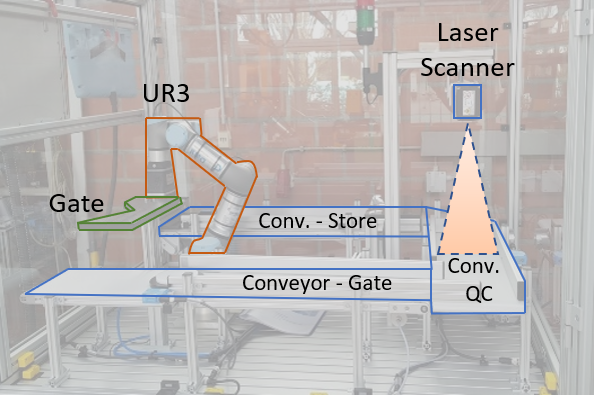
\includegraphics[width=.45\textwidth]{img/demozelle}
       \caption{The industry 4.0 demonstration cell at the University of Siegen}
\label{fig:ind_cell}
\end{figure}

\section{Machine Learning Methods} %3/4 Page

We compare Support Vector Machines (SVM), Multilinear Perceptrons
\cite{bishop2006pattern} as well as random forests in the task of
quality prediction. All three will be introduced next.

\subsection{Multilayer perceptrons}
These feedforward neural networks typically combine multiple layers
and activation functions \cite{bishop2006pattern}.
A layer contains a large weight matrix and
a bias vector. To evaluate the layer the input vector must be
multiplied with the weight matrix before the bias vector is added.
Each layer is typically followed by an activation function 
which adds non-linearity to the network graph. Rectified linear units
(ReLUs) are zero for negative inputs leave positive inputs unchanged.
ReLUs are the recommended activation function for modern neural
networks \cite{goodfellow2016deep} we use these here as well.
Since the linear parts of the ReLU and the linear matrix multiplication
are differentiable we can employ gradient descent to train our 
classifier.

\subsection{Support Vector Machines}
Support Vector Machines (SVM) attempt to separate data
along hyperplanes \cite{aggarwal2015data}. 
SVM offer a convex alternative to MLPs \cite{Suykens2002least}.
A convex classifier is guaranteed to converge to a global solution
regardless of its initialization.
Non-separable data can become separable if projected to a different
possibly high dimensional space trough a Kernel function.
The Kernel trick allows SVM to solve some non-linear
classification problems \cite{Suykens2002least}
Radial basis functions (RBF) are commonly chosen as kernels
\cite{Suykens2002least} we choose to follow this practice as well.

\subsection{Decision Tree}
Decision trees are binary trees, these binary trees work with the input
features at the roots, decisions are made by moving
up the tree to top leaves. At every branch in the tree, a decision
is made, until one arrives at the decision \cite{Marsland2015Machine}.
For numerical input features, each decision partitions the data
\cite{aggarwal2015data}. For example by comparison to a threshold value.
To construct the tree these cutoff values have to be chosen
at every branch. The construction problem turns into an optimization 
problem when a split criterion is introduced. Common choices are 
cross-entropy of Gini-coefficient \cite{aggarwal2015data}.
During construction, the chosen function must be minimized. 


\section{Experiments}

\subsection{Data acquisition}

Industrial projects requires to work with a variety of sensors and controllers. Thus, it might occurs incompatibility between technologies. In order to avoid that problem, universal protocols are often implemented at industrial projects. This is the case for our industrial 4.0 demonstration cell, which shares data via protocol OPC-UA. 

Figure~\ref{fig:robot_pos_cell} describes a simplified version of the real connection diagram of the demonstration cell. For our case, the data is shared independently from two OPC-UA servers. This in order to represent the interaction between multiple servers in real production environments. 

The first step to collect the data is to list all the variables of interest and to map their source. The second step is to determine the use cases of interest.  On this research, we focussed on the data described on Table.~\ref{tab:data_source} and the six use cases described on Table.~\ref{tab:use_cases}. The data was manually collected by using the software "UAExperts". Approximately 15 hours of data was collected, by equally sampling each use case during the data acquisition time.

\begin{table}
       \centering
       \begin{adjustbox}{width=.45\textwidth}
       \begin{tabular}{ c c c } \toprule
              \textbf{Data of interest} & \textbf{Server Source} & \textbf{Variable}\\ \midrule
              Conveyor speed       & Siemens PLC       & \begin{minipage}[t]{0.2\textwidth}
              \begin{description}
                     \item Conveyor: Gate
                     \item Conveyor: QC
                     \item Conveyor: Store
                     \end{description}
                     \end{minipage} \\ \hline
              UR3 Position         & Siemens PLC       & \begin{minipage}[t]{0.2\textwidth}
              \begin{description}
                     \item $xyz$ Gripper position
                     \end{description}
                     \end{minipage} \\ \hline
              Action Flags         & Siemens PLC       & \begin{minipage}[t]{0.2\textwidth}
              \begin{description}
                     \item UR3 gripper open/close
                     \item Grab/drop disk based on disk type
                     \end{description}
                     \end{minipage} \\ \hline
              Quality control      & SICK SIM4000      & \begin{minipage}[t]{0.2\textwidth}
              \begin{description}
                     \item OK-NOK label
                     \item $xy$ disk deviation from the center point
                     \item Absolute disk deviation
                     \end{description}
                     \end{minipage} \\ \hline
              Gate position        & SICK SIM4000      & \begin{minipage}[t]{0.2\textwidth}
              \begin{description}
                     \item Position
                     \item Speed
                     \item Safe to go
                     \end{description}
                     \end{minipage} \\ \hline
              Store       & SICK SIM4000      & \begin{minipage}[t]{0.2\textwidth}
                     \begin{description}
                     \item Disk Size
                     \end{description}
                   \end{minipage} \\ \bottomrule
       \end{tabular}
       \end{adjustbox}
       \caption{Industriy 4.0 demonstration cell: Relevant data with its reference source server}
       \label{tab:data_source}
\end{table}

\begin{table}
       \centering
       \begin{tabular}{ c c } \toprule
              Use Case        & Description \\ \midrule
              Use Case 1  & \begin{minipage}[t]{0.25\textwidth}
                            \begin{description}
                                   \item Conveyor speed: Slow
                                   \item Robot position: OK
                            \end{description}
                            \end{minipage}  \\ \hline
              Use Case 2  & \begin{minipage}[t]{0.25\textwidth}
                            \begin{description}
                                   \item Conveyor speed: Slow
                                   \item Robot position: NOK
                            \end{description}
                            \end{minipage}  \\ \hline
              Use Case 3  & \begin{minipage}[t]{0.25\textwidth}
                            \begin{description}
                                   \item Conveyor speed: Fast
                                   \item Robot position: OK
                            \end{description}
                            \end{minipage}  \\ \hline
              Use Case 4  & \begin{minipage}[t]{0.25\textwidth}
                            \begin{description}
                                   \item Conveyor speed: Fast
                                   \item Robot position: NOK
                            \end{description}
                            \end{minipage}  \\ \hline
              Use Case 5  & \begin{minipage}[t]{0.25\textwidth}
                            \begin{description}
                                   \item Conveyor speed: Too Fast
                                   \item Robot position: OK
                            \end{description}
                            \end{minipage}  \\ \hline
              Use Case 6  & \begin{minipage}[t]{0.25\textwidth}
                            \begin{description}
                                   \item Conveyor speed: Too Fast
                                   \item Robot position: NOK
                            \end{description}
                            \end{minipage}  \\ \bottomrule
       \end{tabular}
       \caption{Industrial 4.0 demostration cell: Controlled use-cases.
       Use cases with Robot position: NOK and Conveyor speed: Too Fast will result in NOK pieces.}
       \label{tab:use_cases}
\end{table}


\begin{figure}
       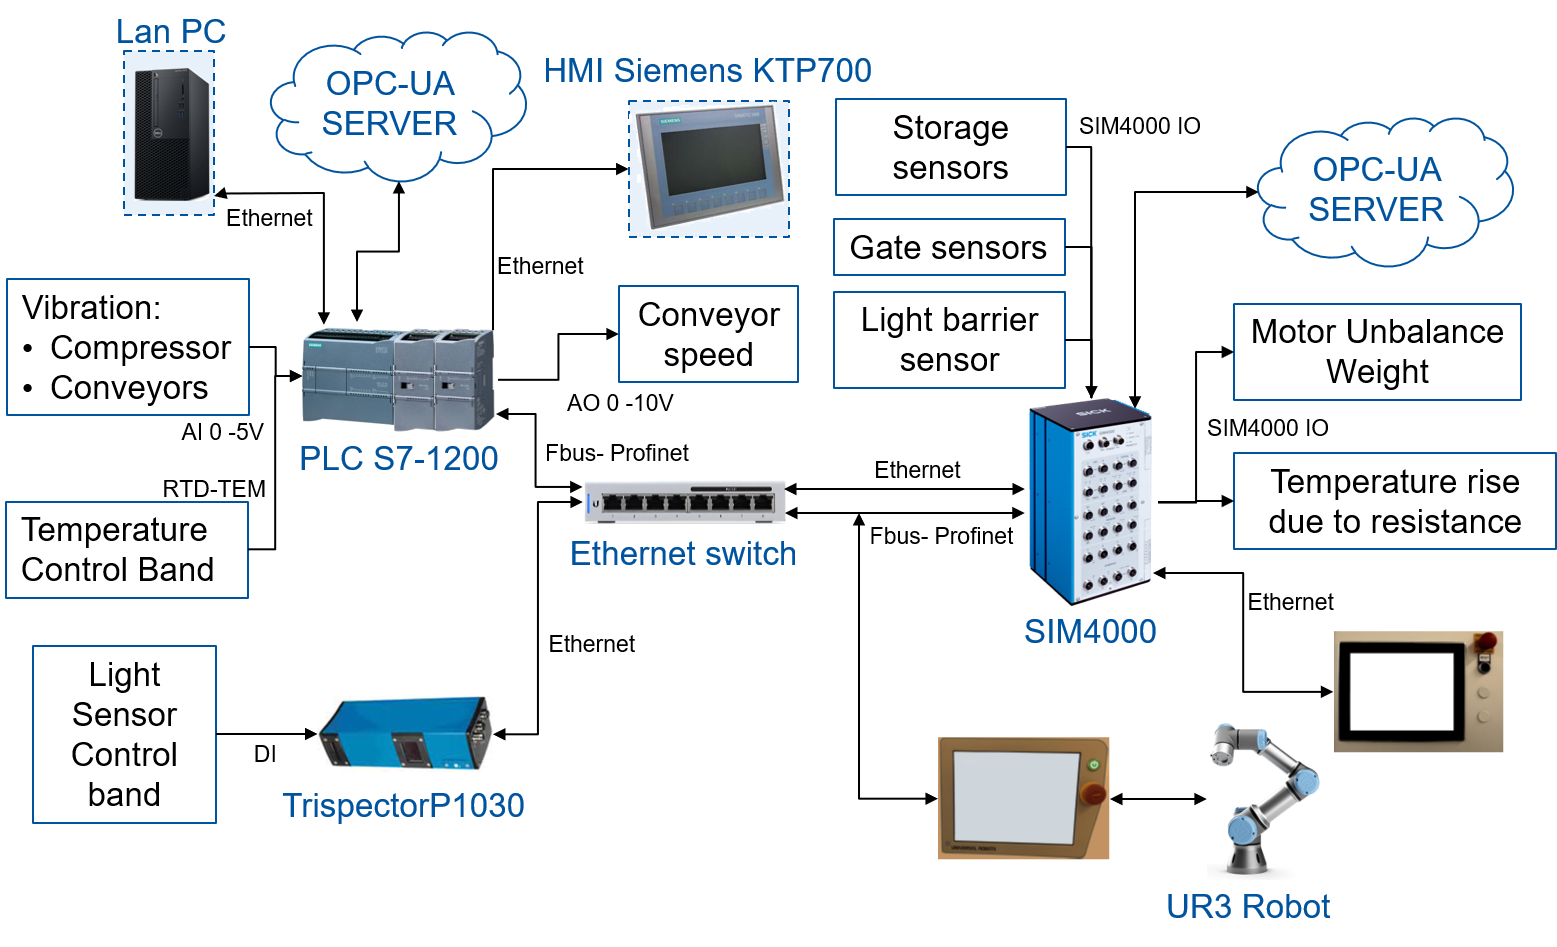
\includegraphics[width=.45\textwidth]{img/demozelle_conex_diagram.png}
       \caption{Industry 4.0 demostration cell: Connection diagram (simplified)
             }
\label{fig:demo_conn_diag}
\end{figure}

\subsection{Data preprocessing}

Once enough data is collected, the next step is to clean the raw data and organize it accordingly. For our case, that means to merge the data collected from the two OPC-UA servers, synchronize the time stamps. Since our systems are not completely synchronized, it was needed to calculate the delta-time based between servers based on the base clock from each server. Once the delta-time was determined, a time-stamp function was implemented to correct the time-shift between samples and be able to merge all the data without incompatibilities.

Data tags interpretation is an important step in the preprocessing process. The raw data collected from the sensors is sometimes tagged by an alphanumeric code. In order to work with the data, it was needed to implement diverse functions wich have the task to clean the raw data in a more human-readable form. This means to remove samples out of clear boundaries and missing values, as well as to translate the sensors code based in a predefined dictionary settle by the authors. This last step, could be optional in other implementations, however, it proves to be a great addition for testing purposes.

Once the data is clean and compiled in one directory, the next step would be to split the data based on the assembly cycle. For our purposed, we split the dataset in individual data-samples with help of the action tags included in the dataset Table.~\ref{tab:data_source}. Subsequently, each data-sample is automatically checked for missing sensor values and diskarded if so. At this point we have a series de data-samples, which each of them is based in time series. However, we are not interested in a time series analysis, therefore it would be needed to compress each time-series based data-sample in an atemporal data-sample.

To eliminate time as a variable in our dataset, we defined a series of rules:

\begin{itemize}
       \item Robot position ($xyz$) while dropping the disk in the storage area
       \item Mean conveyor speed per conveyor band
       \item Absolute deviation ($xy$) at the quality control check
       \item Absolute quality check result: OK - NOK
\end{itemize}

Each time-series sample was evaluated based on the rules stated above, and the result of each evaluation was considered as our atemporal data-sample, which would be used by our classifier.

\subsection{Classifier optimization and testing}\label{sec:ml_exp}

\begin{figure}
       \includestandalone[width=.45\textwidth]{img/arm_data_plot}
       \caption{Robot arm movement patterns. We show the movement of the 
                cell's robot arm, its grippers, and the encoding of the overall
                position in the system. The changes in the grip flag are triggered,
                when the gripper opens or closes. Zero indicates an open, while
                one indicates a closed gripper. The position flags marks the state
                of the cell's arm. 0 means the black disk is in store,
                one that the black disk is at the gate, two that the white disk
                is in store and three that the white disk is located at the gate.
             }
\label{fig:robot_pos_cell}
\end{figure}

The robot's position at disk drop is marked in 
Figure~\ref{fig:robot_pos_cell}. The quality prediction problem is 
framed as a classification task. The input vectors which we feed into our
classifiers consists of the arm positions at the disk drops for both
disks in three dimensions, as well as the largest recorded belt speed
of all three belts. The interpretation of the quality measurement is 
used as the training target. It can be good or bad which we encode as 
zero and one.

We work with a total of 528 measurements. Each containing arm and belt data
logs of individual cell runs. 50 samples are set aside at random for testing 
purposes, leaving 478 training samples. The random number generator seed is
set to one to ensure the train and test set splits are identical 
for all experiments.

We compare a total of three different classifier architectures on the data.
A Support Vector Machine (SVM), a multilinear perceptron (MLP) and a Random Forest
structure. All three methods are trained using standard hyperparameters.
\footnote{In order to allow exact reproduction of these results source
code is available at \url{https://github.com/manubrain/Demo-Cell-Classification}}

\begin{table}
       \centering
       \begin{tabular}{ c c } \toprule
              Approach         & accuracy \\ \midrule
              Na\"ive-Baseline & 64 \% \\
              Support Vector Machine & 82 \% \\
              Multilayer Perceptron & 88 \% \\
              Decision Tree         & 98 \% \\ \bottomrule
       \end{tabular}
       \caption{Comparison of Support Vector Machine (SVM), Multilinear Perceptron and 
                Random Forest classification on our anomaly detection task. 
                The first row shows the performance of naively predicting a broken piece
                every time.}
       \label{tab:class_comp}
\end{table}

\begin{table}
       \begin{subtable}[h]{0.3\textwidth}
              \centering
              \begin{adjustbox}{width=1.6\textwidth}
              \begin{tabular}{l|l|c|c|c}
                     \multicolumn{2}{c}{}&\multicolumn{2}{c}{True Values}&\\
                     \cline{3-4}
                     \multicolumn{2}{c|}{}& OK & NOK &\multicolumn{1}{c}{Total}\\
                     \cline{2-4}
                     \multirow{2}{*}{Predicted Values}& OK & $18$ & $0$ & $18+0 = 18$\\
                     \cline{2-4}
                     & NOK & $8$ & $24$ & $8+24 = 32$\\
                     \cline{2-4}
                     \multicolumn{1}{c}{} & \multicolumn{1}{c}{Total} & \multicolumn{1}{c}{$18+8 = 26$} & \multicolumn{    1}{c}{$0+24 = 24$} & \multicolumn{1}{c}{$50$}\\
              \end{tabular}
              \end{adjustbox}
              \caption{SVM.}
              \label{tab:SVM_conf_matrix}
       \end{subtable}
       \begin{subtable}[h]{0.3\textwidth}
              \centering
              \begin{adjustbox}{width=1.6\textwidth}
              \begin{tabular}{l|l|c|c|c}
                     \multicolumn{2}{c}{}&\multicolumn{2}{c}{True Values}&\\
                     \cline{3-4}
                     \multicolumn{2}{c|}{}& OK & NOK &\multicolumn{1}{c}{Total}\\
                     \cline{2-4}
                     \multirow{2}{*}{Predicted Values}& OK & $18$ & $0$ & $18+0 = 18$\\
                     \cline{2-4}
                     & NOK & $6$ & $26$ & $6+26 = 32$\\
                     \cline{2-4}
                     \multicolumn{1}{c}{} & \multicolumn{1}{c}{Total} & \multicolumn{1}{c}{$18+6 = 24$} & \multicolumn{    1}{c}{$0+26 = 26$} & \multicolumn{1}{c}{$50$}\\
              \end{tabular}
              \end{adjustbox}
              \caption{MLP.}
              \label{tab:MPL_conf_matrix}
       \end{subtable}
       \begin{subtable}[h]{0.3\textwidth}
              \centering
              \begin{adjustbox}{width=1.6\textwidth}
              \begin{tabular}{l|l|c|c|c}
                     \multicolumn{2}{c}{}&\multicolumn{2}{c}{True Values}&\\
                     \cline{3-4}
                     \multicolumn{2}{c|}{}& OK & NOK &\multicolumn{1}{c}{Total}\\
                     \cline{2-4}
                     \multirow{2}{*}{Predicted Values}& OK & $17$ & $1$ & $17+1 = 18$\\
                     \cline{2-4}
                     & NOK & $0$ & $32$ & $0+32 = 32$\\
                     \cline{2-4}
                     \multicolumn{1}{c}{} & \multicolumn{1}{c}{Total} & \multicolumn{1}{c}{$17+0 = 17$} & \multicolumn{    1}{c}{$1+32 = 33$} & \multicolumn{1}{c}{$50$}\\
              \end{tabular}
              \end{adjustbox}
              \caption{Decision Tree.}
              \label{tab:Tree_conf_matrix}
       \end{subtable}
       \caption{Confusion matrix result of the prediction of 50 data-points.}
       \label{tab:Confusion_matrix}
\end{table}


Results are shown in table~\ref{tab:class_comp}. For 32 of the total 50 test samples
quality measurements indicate a problem. This sets the 
baseline over the entire data set, which would be obtained by simply labeling all samples
as faulty. Over the test set, we require to classify more than 64\% of the data correctly.
We would therefore expect any naive classifier to produce at least 64\% accuracy, which we have to beat. In Table~\ref{tab:class_comp}, we observe that this is indeed the case for all three approaches evaluated here.

Based on the MLP prediction results presented on Table.~\subref{tab:MPL_conf_matrix} shows that even though the prediction model is not 100\% accurate, the percentage of false-positive predictions is 0\%. The false-negative results represents the 12\% of the test sample and the true predictions constitute 88\% of the test data.

The outcome of the models shows that the random forest performed best followed by the multilinear perceptron and the support vector machine. However, by reviewing the confusion matrices presented on Table,~\ref{tab:Confusion_matrix}, multilinear perceptron would be the option of choice to be implemented at industrial applications due to the 0\% ratio in false-positive results.

\section{Conclusion}

% Quality assurance is an important topic in production. Quality assurance methods in production might diverge one from each other, however, all of them seek to prove the product quality in one way or another. 

Based on the literature review, we observed that the hundred percent quality check method proves to be the most efficient method to guarantee the final product quality, however, the high implementation cost is its biggest draw back. On the other hand, we have the statistical methods, which are known to be fast and efficient, but the lack of reviewing each individual product until the next bach review might imply a considerable loss whenever NOK products are found. This based in the uncertainty of when did the error occurs and how many products are affected.

By implementing ML models capable to predict the quality of the product, just by the initial conditions of the process would be a great asset for the industrial processes. Within the limits of our work, we are able to predict with 98\% certainty the product quality by implementing a decision tree model with a 6-variables vector as input. 
However, our decision for industrial applications would be the MLP with 88\% accuracy as to guarantee the QC and avoid labeling a NOK piece as OK. For further work, we expect to increase the certainty of the prediction model by collecting more data-samples and experimenting with other, more complex, ML models.

It is important to state that this prediction model is not yet ready to fully replace the statistical methods, not the hundred percent quality check method. However, a combination of SPC along prediction models could work well together, since the prediction model will evaluate each produced piece, and this will somehow compensate one of the disadvantages from statistical methods.

It is worth to mention the most important points learned during the project implementation. This might help as building blocks for further research in the area.

\subsection{Lesson Learned} % 1/2 Page

\textbf{Incompatibility between technologies}; devices configured on the same network presented troubles to share data within each other due to network restrictions, as well as the limitation to access and modify restricted program-code given by the machine manufacture. 
To overcome the situation stated above, it was necessary to reprogram big sections of the machine control system.

\textbf{Data synchronization}; two OPC-UA servers were used on this implementation. This lead to a series of data synchronization problems due to differences on the internal clock of both servers.
In order to solve the issue, it was needed to write a time-stamp synchronization script that was deployed during the data preprocessing phase. Without harmonious time-stamps, the input data for the ML model would have been useless and the model inaccurate. 

\textbf{Data interpretation}; complex, time-consuming, and fundamental step on any ML applications. It is fundamental to understand the assembly process, the timing from the machine movements, the boundaries of the machine's sensors, as well of a basic correlation within the presented data.

\textbf{Missing values}; in order to minimize the risk of false results delivered by the ML model, it would be compulsory to carefully review the ML input data. Missing values can have a great impact in the ML prediction, that is the reason why we deliberately review all the input data and validate it with the expected output from the diverse sensors. Whenever there was missing data, and as long as we did not fabricate data, we employed statistical methods to fill the data gap.

\textbf{Adapting the industry 4.0 demonstration cell}; the initial state of the demonstrator was very limited. Even though the process was well known, the lack of labels or flags whenever certain actions occurs, made complicated to have accurate data sampling from each assembly cycle. In order to overcome this uncertainty, we modify the machine program to raise specify flags whenever certain actions would be executed.

\textbf{Machine Learning}; careful measurement and  meaningful preprocessing
of our cell-date was key to the successful application of all three algorithms.
Without the labels the problem could not have been framed as a supervised 
classification problem.

\textbf{Dataset size}; as the starting point we collected as many data points as the ones found in the iris Dataset \cite{fisher_1936}. The next step was to collect batches of data of around 30 minutes per use case. This process was repeated until accumulate around 15 hours of data.

\section*{Acknowledgments}
This project was partly supported by the German and European IKT.NRW
project "`ManuBrain"' 

\bibliographystyle{abbrv}
\bibliography{bib}

\end{document}
